%! Mode:: "TeX:UTF-8"
%! TEX program = xelatex
\PassOptionsToPackage{quiet}{xeCJK}
\documentclass[withoutpreface,notoc]{cumcmthesis}

% === 建议在此处加载 cls 文件未包含的、个人需要的宏包 ===
% 使用 natbib 的 super 选项实现上标引用
\usepackage[super,numbers,sort&compress]{natbib}
\usepackage[framemethod=TikZ]{mdframed} % 框架宏包
\usepackage{pdfpages} % 插入pdf页面

% === 建议在此处进行全局格式设置 ===
\usepackage{etoolbox}
% 将表格内的字体全局设置为五号
\BeforeBeginEnvironment{tabularx}{\zihao{5}}

% === 自定义表格列类型 ===
\newcolumntype{C}{>{\centering\arraybackslash}X}
\newcolumntype{R}{>{\raggedleft\arraybackslash}X}
\newcolumntype{L}{>{\raggedright\arraybackslash}X}
% 自动分配宽度的说明列
\newcolumntype{Y}{>{\centering\arraybackslash}X} % 左对齐,可伸缩
\newcolumntype{S}{>{\centering\arraybackslash}m{2cm}} % 固定宽度 2cm,居中

\title{基于是谁的的是多少是多少沙发上的模型} % 论文标题

%%%%%%%%%%%%%%%%%%%%%%%%%%%%%%%%%%%%%%%%%%%%%%%%%%%%%%%%%%%%%
%% 正文
\begin{document}
	\maketitle
    \thispagestyle{plain}
	\begin{abstract}
		摘要是论文的门面,需要高度概括你的工作。清晰地说明你们针对每个问题所采用的核心模型和关键算法,以及得到的主要结论和模型的亮点。
		
		\textbf{针对问题一,} 我们建立了...模型,通过...方法求解,得到了...的结果。
		
		\textbf{针对问题二,} 我们应用了...算法,分析了...,发现...。
		
		\textbf{针对问题三,} 我们创新性地提出了...,其优点在于...。
		
		\textbf{针对问题四,} ...
		
		最后,本文的模型具有较好的鲁棒性和可扩展性。
        这里试试换行!
		
		\keywords{关键词\quad 关键词\quad 关键词\quad 关键词 \quad 关键词}
	\end{abstract}
	%%%%%%%%%%%%%%%%%%%%%%%%%%%%%%%%%%%%%%%%%%%%%%%%%%%%%%%%%%%%%
	
	% 国赛最终提交版本通常不包含目录页
	% \tableofcontents
	% \newpage
	
	%%%%%%%%%%%%%%%%%%%%%%%%%%%%%%%%%%%%%%%%%%%%%%%%%%%%%%%%%%%%%
	% 建议:第一节使用“问题重述”更符合竞赛范式
	\section{问题重述}
	在此部分简要重述赛题,厘清需要解决的关键问题点。这能向评委展示你对问题的理解是准确且深入的。
    \subsection{问题一}
    \subsubsection{首先}
	
	%%%%%%%%%%%%%%%%%%%%%%%%%%%%%%%%%%%%%%%%%%%%%%%%%%%%%%%%%%%%%
	\section{模型假设}
	为简化问题,便于模型建立与求解,本文做出以下合理假设:
	\begin{itemize}[itemindent=2em]
		\item \textbf{假设1:} 这是一个非常重要的假设...
		\item \textbf{假设2:} 我们假设所有数据均是可靠且无误差的...
		\item \textbf{假设3:} 暂不考虑...等次要因素的影响。
	\end{itemize}
	
	%%%%%%%%%%%%%%%%%%%%%%%%%%%%%%%%%%%%%%%%%%%%%%%%%%%%%%%%%%%%%
	\section{符号说明}
	为方便阅读,本文使用的主要符号及其说明如\cref{tab:符号说明}所示。
	\begin{table}[H]
		\centering
		\caption{符号说明表} % 建议为所有图表添加标题
		\label{tab:符号说明}
		\begin{tabularx}{\textwidth}{SYS}
			\toprule
			符号 & 说明 & 单位 \\
			\midrule
			$m$ & 质量 & kg \\
			$g$ & \text{次品率为$p$的整批产品,选取抽样数为$n$,则其中次品件数$v\leq c$的概率} & m/s$^2$ \\
			$\alpha$ & 某个角度 & rad \\
			\bottomrule
		\end{tabularx}
	\end{table}
	
	%%%%%%%%%%%%%%%%%%%%%%%%%%%%%%%%%%%%%%%%%%%%%%%%%%%%%%%%%%%%%
	\section{问题一的模型建立与求解}
	\subsection{模型建立}
	根据题意和相关物理定律,我们可以建立...模型。
	\begin{lemma}
		这是一个引理...
	\end{lemma}
	\begin{definition}
		这是一个定义...
	\end{definition}
	
	% 建议:使用 \[...\] 代替 $$...$$
	\[
	E = mc^2
	\]
	
	这是一个需要引用的重要公式,见\cref{eq:爱因斯坦质能方程}。
	\begin{equation}
		\label{eq:爱因斯坦质能方程}
		E = mc^2
	\end{equation}
	
	下图 (\cref{fig:单图}) 展示了一个示例。
	\begin{figure}[ht]
		\centering
		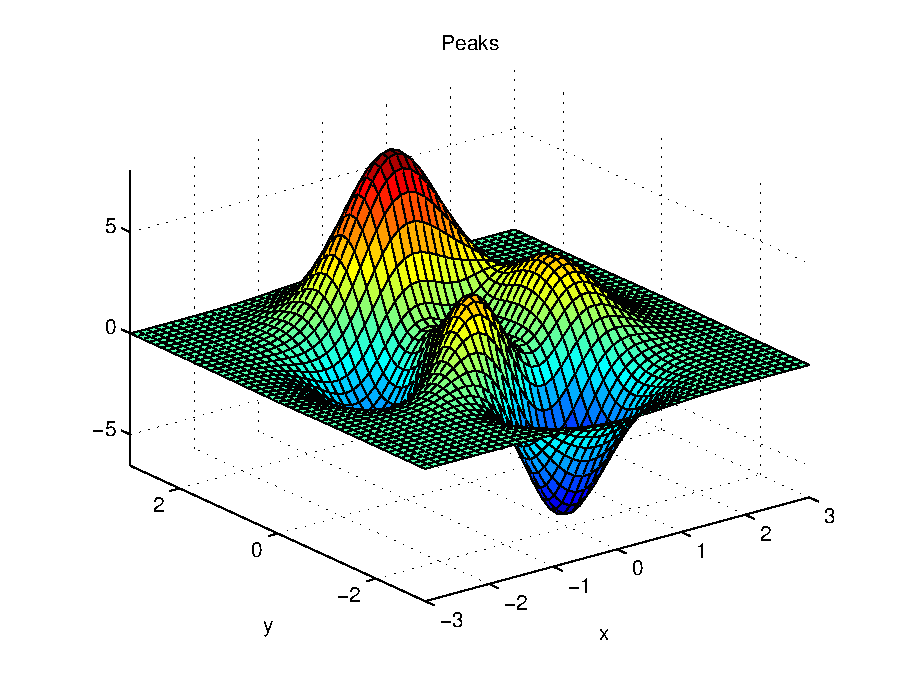
\includegraphics[width=0.7\textwidth]{example.eps} % example.eps 是一个占位图
		\caption{单图示例}
		\label{fig:单图}
	\end{figure}
	
	这句话引用了文献\cite{司守奎2011数学建模算法与应用}。现在所有引用都将自动变为上标。
	
	\subsection{模型求解}
	    为求解上述模型,我们设计了如下步骤:这里是测试赛试试这里是测试赛试试这里是测试赛试试这里是测试赛试试

        这里是测试赛试试

        % 这个东西格式不是很好,弃用
        % \begin{description}
        % 	\item[Step 1:] 数据预处理...这是第一步的说明,数据预处理摘要是论文的门面,需要高度概括你的工作。清晰地说
        % 	\item[Step 2:] 利用 MATLAB/Python 实现...算法...
        % 	\item[Step 3:] 结果后处理与可视化...
        % \end{description}

        % 直接手敲
        \textbf{Step 1:} 数据预处理...这是第一步的说明,数据预处理摘要是论文的门面,需要高度概括你的工作。清晰地说

        \textbf{Step 2:} 数据预处理...这是第一步的说明,数据预处理摘要是论文的门面,需要高度概括你的工作。清晰地说

        \textbf{Step 3:} 数据预处理...这是第一步的说明,数据预处理摘要是论文的门面,需要高度概括你的工作。清晰地说

    \begin{enumerate}
        \item 首先,...。
        \item 其次,...。
        \item 最后,...。
    \end{enumerate}


	\subsection{求解结果与分析}

	这是一个需要引用的重要公式,见\cref{eq:动能定理}。
	\begin{equation}
		\label{eq:动能定理}
		E = \frac{1}{2}mv^2
	\end{equation}
	
	%%%%%%%%%%%%%%%%%%%%%%%%%%%%%%%%%%%%%%%%%%%%%%%%%%%%%%%%%%%%%
	\section{问题二的模型建立与求解}
	\subsection{模型建立}
	对于问题二,我们考虑...因素,建立了...模型。如\cref{fig:双图}所示,其中\cref{fig:双图a}展示了...,\cref{fig:双图b}展示了...。
	
	\begin{figure}[ht]
		\centering
		\subcaptionbox{子图A的标题\label{fig:双图a}}
		{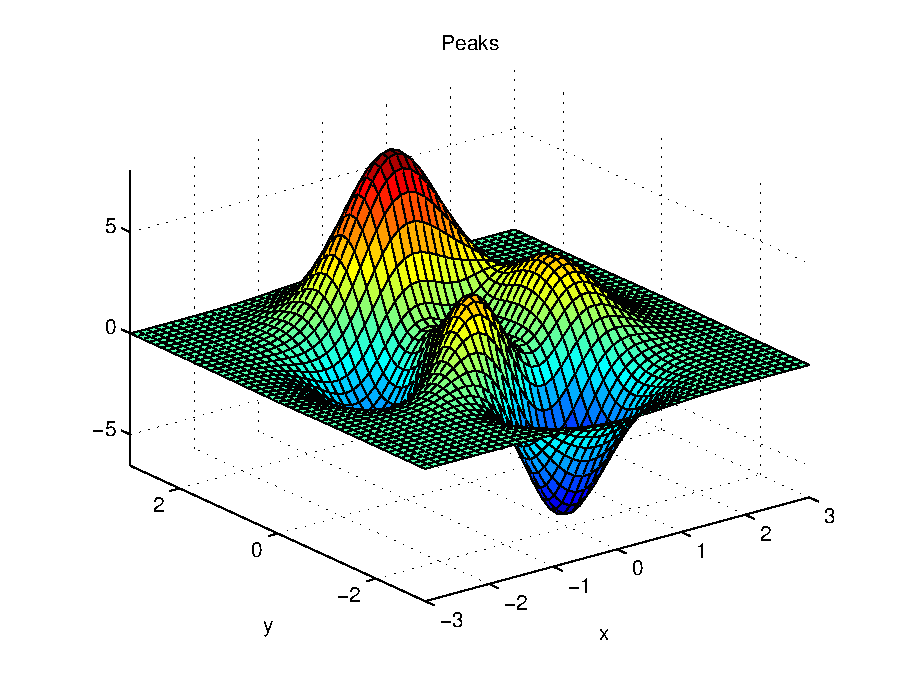
\includegraphics[width=.45\textwidth]{example.eps}}
		\hfill % 让两个子图尽可能分开
		\subcaptionbox{子图B的标题\label{fig:双图b}}
		{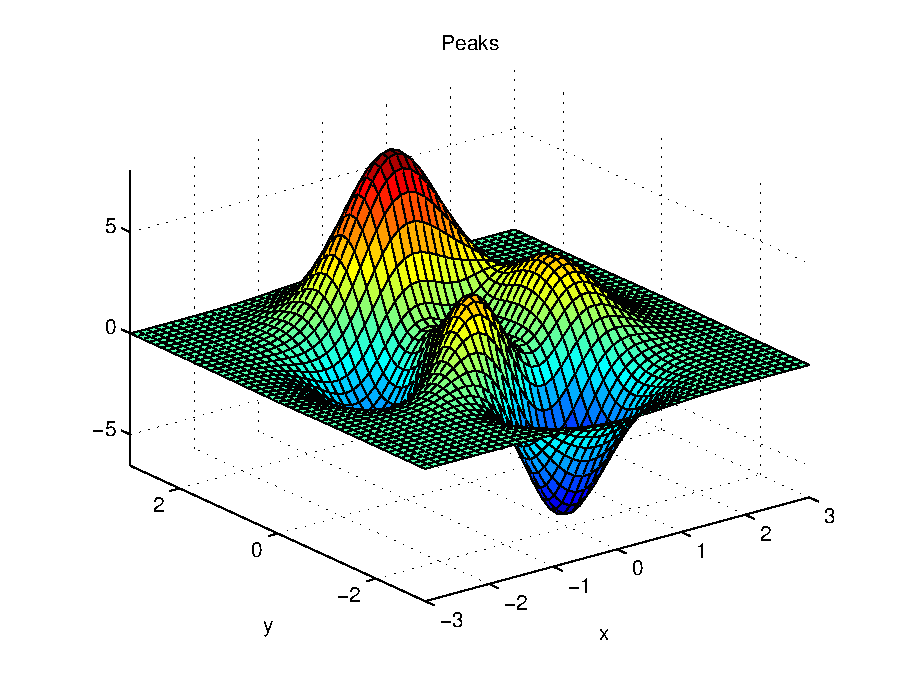
\includegraphics[width=.45\textwidth]{example.eps}}
		\caption{双子图示例}
		\label{fig:双图}
	\end{figure}
	
	% ... 后续问题类似 ...
	\section{模型的分析与检验}
	\subsection{灵敏度分析}
	...
	\subsection{误差分析}
	...
	%%%%%%%%%%%%%%%%%%%%%%%%%%%%%%%%%%%%%%%%%%%%%%%%%%%%%%%%%%%%%
	\section{模型的评价与推广}
	\subsection{模型的优点}
	\begin{itemize}[itemindent=2em]
		\item \textbf{优点1:}模型结构简洁,物理意义明确。模型结构简洁,物理意义明确。模型结构简洁,物理意义明确。模型结构简洁,物理意义明确。模型结构简洁,物理意义明确。
		\item \textbf{优点2:}算法效率高,求解速度快。
		\item \textbf{优点3:}模型具有较好的通用性,可推广至...
	\end{itemize}
	\subsection{模型的缺点}
	\begin{itemize}[itemindent=2em]
		\item \textbf{缺点1:}假设条件较强,在...情况下可能失效。
		\item \textbf{缺点2:}未考虑...因素,与实际情况存在一定偏差。
	\end{itemize}
	
	%%%%%%%%%%%%%%%%%%%%%%%%%%%%%%%%%%%%%%%%%%%%%%%%%%%%%%%%%%%%%
	%% 参考文献
	% 建议:最终提交时删除 \nocite{*}
	% \nocite{*}
	\bibliographystyle{gbt7714-numerical} % 引用格式,符合国标
	\bibliography{ref} % 你的 .bib 文件名,这里假设是 ref.bib
	
	\newpage
	%%%%%%%%%%%%%%%%%%%%%%%%%%%%%%%%%%%%%%%%%%%%%%%%%%%%%%%%%%%%%
	%% 附录
	\begin{appendices}
		\section{支撑材料列表}
		\begin{table}[H]
			\centering
			\caption{附录文件列表}
			\label{tab:文件列表}
			\begin{tabularx}{\textwidth}{LL}
				\toprule
				文件名 & 功能描述 \\
				\midrule
				q1.m & 问题一核心 MATLAB 程序代码 \\
				q2.py & 问题二 Python 求解程序 \\
				data.xlsx & 本文使用的原始数据与处理结果 \\
				\bottomrule
			\end{tabularx}
		\end{table}
		
		\section{核心代码}
		\noindent\textbf{问题一 MATLAB 代码 (q1.m)}
		\lstinputlisting[language=matlab]{code/q1.m}
		
		\noindent\textbf{问题二 Python 代码 (q2.py)}
		\lstinputlisting[language=python]{code/q2.py}
		
	\end{appendices}
	
\end{document}